\documentclass{ieeeaccess}
\usepackage{cite}
\usepackage{amsmath,amssymb,amsfonts}
\usepackage{algorithmic}
\usepackage{graphicx}
\usepackage{textcomp}
\usepackage{multirow}
\usepackage{ulem}
\usepackage{hyperref}

\def\BibTeX{{\rm B\kern-.05em{\sc i\kern-.025em b}\kern-.08em
    T\kern-.1667em\lower.7ex\hbox{E}\kern-.125emX}}
\begin{document}
% orcid: 0000-0002-9883-3355
\begin{IEEEbiography}[{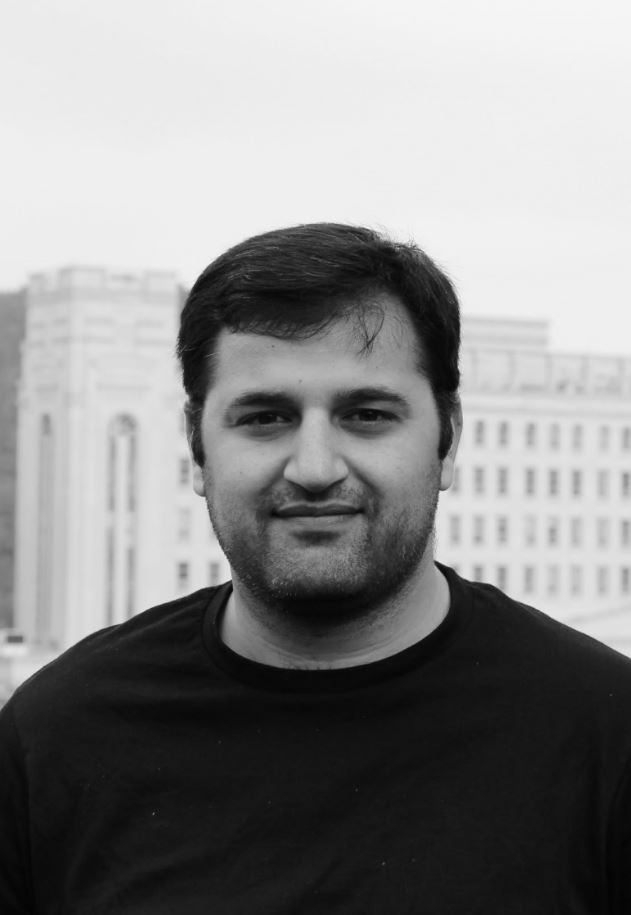
\includegraphics[width=1in,height=1.25in,clip,keepaspectratio]{fahad.jpg}}]{Fahad Ahmed Satti} is currently pursuing Ph.D. in Computer Engineering from Kyung Hee University, South Korea. He completed his MS in Computer Science from University of Trento, Italy in 2014. His primary research interest is directed towards providing a technical solution to resolve the lack of interoperability in information systems. In general, he is interested in domains of semantic matching, stream reasoning, knowledge extraction, and machine learning.
\end{IEEEbiography}
% orcid: 0000-0003-4494-1593
\begin{IEEEbiography}[{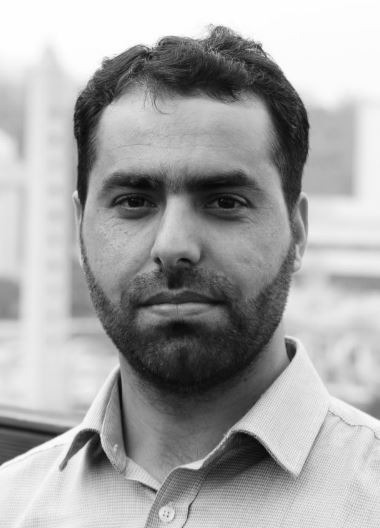
\includegraphics[width=1in,height=1.25in,clip,keepaspectratio]{musarrat.jpg}}]{Musarrat Hussain} is a Ph.D. candidate in the Ubiquitous Computing Laboratory, Kyung Hee University, 	South Korea. He has completed his MS software Engineering in 2015 from National University of Science 	and Technology (NUST) Pakistan. His research interests include clinical text mining, knowledge 	extraction and representation, and machine learning.
\end{IEEEbiography}
% orcid: 0000-0003-3862-8787
\begin{IEEEbiography}[{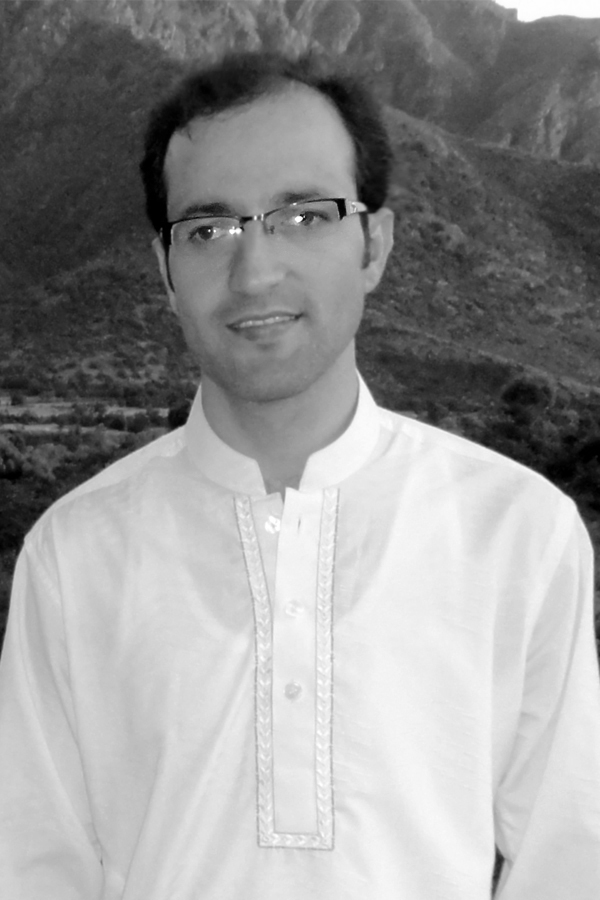
\includegraphics[width=1in,height=1.25in,clip,keepaspectratio]{jamil.jpg}}]{Jamil Hussain} received the Ph.D. degree from the Department of Computer Engineering, Kyung Hee University, South Korea in 2019. He worked as a postdoctoral researcher in the Ubiquitous Computing Laboratory, Kyung Hee University, South Korea, from Sep 2019 to Feb 2021. He is currently an Assistant Professor at Sejong University, South Korea. He has professional experience of over 7 years in the software industry, working on user experience design and development on various projects. His research interest includes user experience design, artificial intelligence, and information extraction from textual data.
\end{IEEEbiography}
% orcid: 0000-0001-8450-6946
\begin{IEEEbiography}[{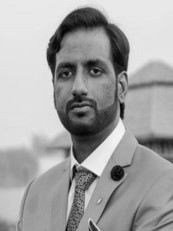
\includegraphics[width=1in,height=1.25in,clip,keepaspectratio]{imran.jpg}}]{Syed Imran Ali} received the BS degree in Computer Science from IQRA University, Islamabad in 2008 and MS degree in Computer Science From National University of Computer and Emerging Sciences (NUCES) in 2012. He has taught in NUCES as an adjunct faculty. He is currently pursuing Ph.D. degree from Department of Computer Science and Engineering, Kyung Hee University, South Korea. His area of interests include machine learning, health analytics and data-driven systems.
\end{IEEEbiography}
% orcid: 0000-0001-8450-6946
\begin{IEEEbiography}[{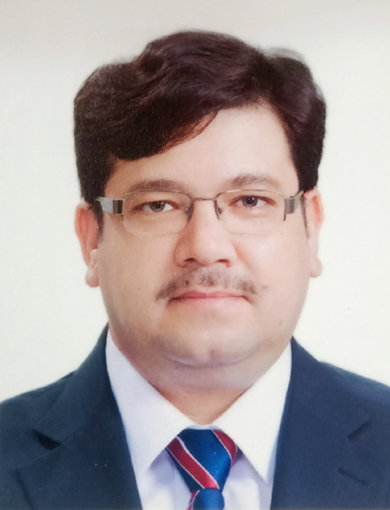
\includegraphics[width=1in,height=1.25in,clip,keepaspectratio]{taqdir.jpg}}]{Taqdir Ali} received the Ph.D. degree from the Department of Computer Engineering, Kyung Hee University, South Korea in 2019. He is currently working as a postdoctoral researcher in the Ubiquitous Computing Laboratory, Kyung Hee University, South Korea. From 2006 to 2011, he was a Senior Software Engineer, a System Analyst, and a Researcher in a reputable software house. His current research includes knowledge acquisition for clinical decision support systems, applications of machine learning, text processing, and e-health standardization.
\end{IEEEbiography}
% orcid: 0000-0002-8920-4231
\begin{IEEEbiography}[{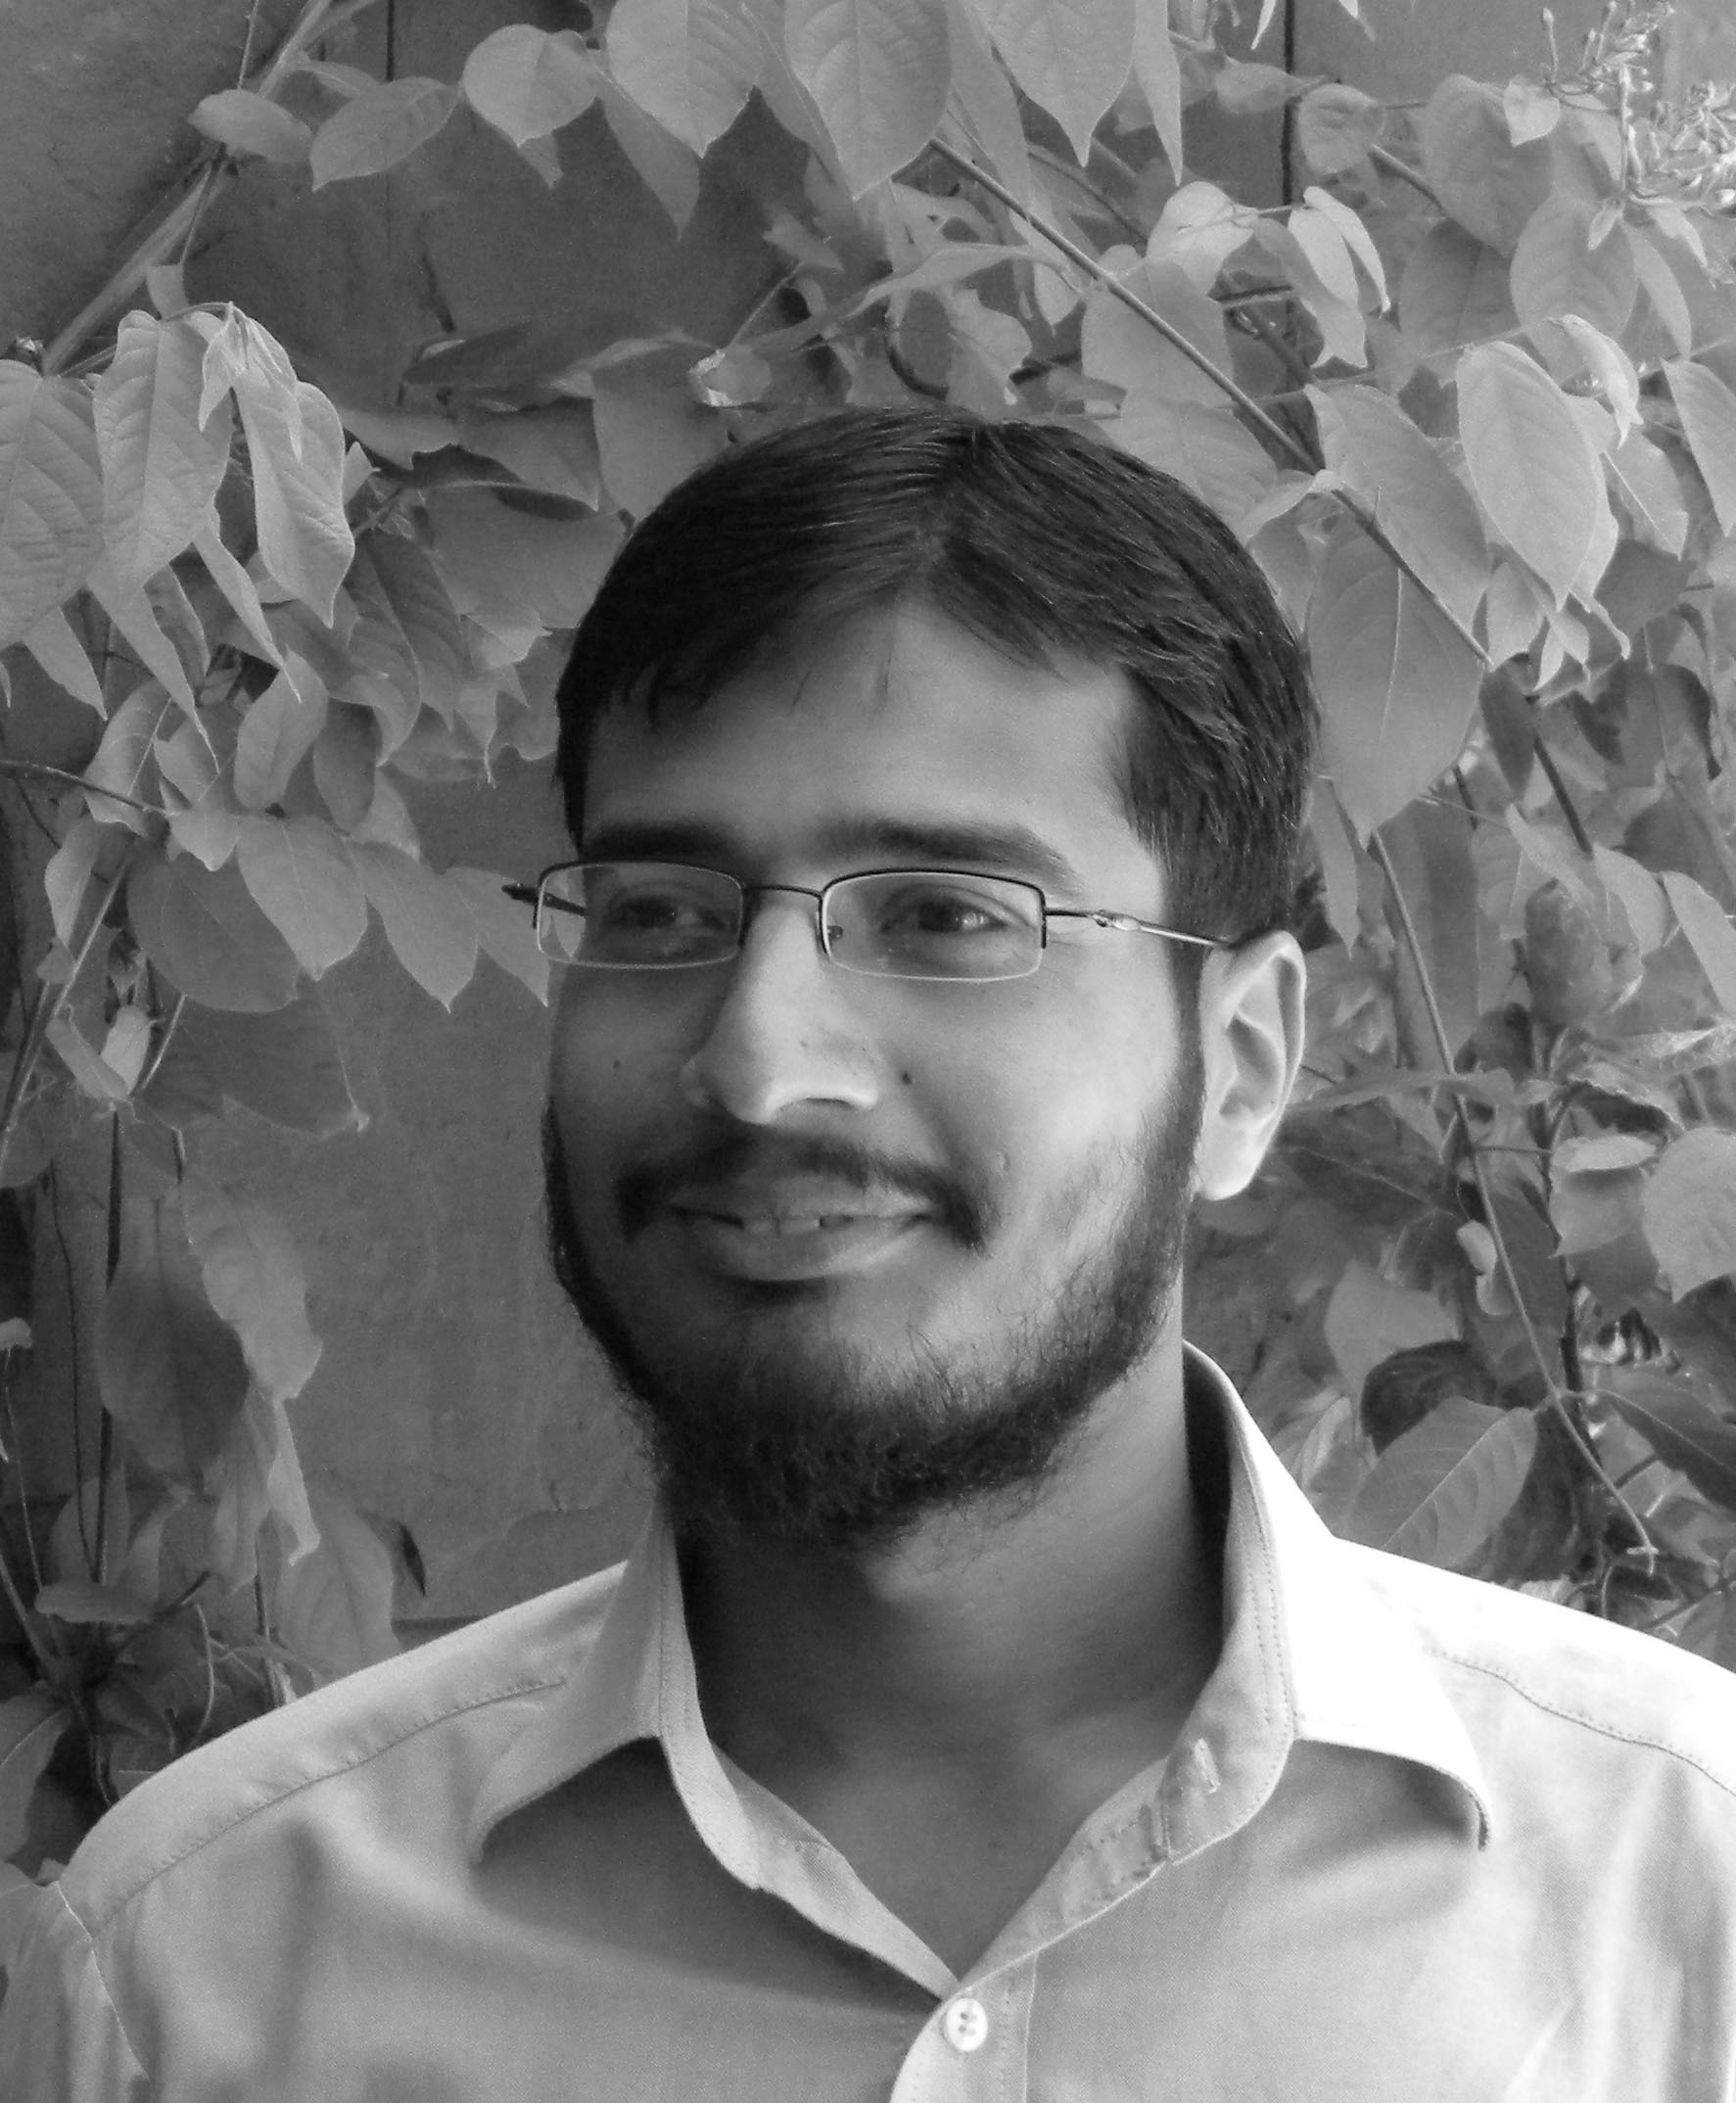
\includegraphics[width=1in,height=1.25in,clip,keepaspectratio]{bilal.jpg}}]{Hafiz Syed Muhammad Bilal}  received the M.S. degree in computer science from National University of Sciences and Technology, Pakistan,in 2008. He is currently pursuing the Ph.D. degree in computer science and engineering at Kyung Hee University, South Korea. He has working experience of more than three years in data science and open source development and is actively involved in developing big data ecosystem for academic and health care. His research interests include behavior quantification \& assessment, machine learning, and behavior modeling \& adaptation.
\end{IEEEbiography}
\begin{IEEEbiography}[{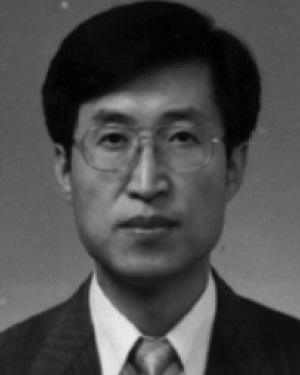
\includegraphics[width=1in,height=1.25in,clip,keepaspectratio]{prof_tcc.jpg}}]{Tae-Choong Chung}  received his B.S. degree in Electronic Engineering from Seoul National University, Republic of Korea, in 1980, and his M.S. and Ph.D. degrees in Computer Science from KAIST, Republic of Korea, in 1982 and 1987, respectively. Since 1988, he has been with the Department of Computer Science and Engineering, Kyung Hee University, Republic of Korea, where he is now a Professor. His research interests include machine learning, meta search, and robotics.
\end{IEEEbiography}
% orcid: 0000-0002-5962-1587
\begin{IEEEbiography}[{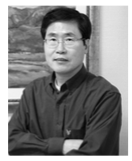
\includegraphics[width=1in,height=1.25in,clip,keepaspectratio]{prof_sylee.png}}]{Sungyoung Lee} received the B.S.degree from Korea University, Seoul, South Korea,and the M.S. and Ph.D. degrees in computer science from the Illinois Institute of Technology,Chicago, IL, USA, in 1987 and 1991, respectively.He was an Assistant Professor with the Department of Computer Science, Governors State University, University Park, IL, USA, from 1992 to 1993. He has been a Professor with the Department of Computer Engineering, Kyung Hee University,South Korea, since 1993, where he has been the Director of the Neo Medical ubiquitous-Life Care Information Technology Research Center since 2006.He is currently the Founding Director of the Ubiquitous Computing Laboratory. His current research interests include ubiquitous computing and applications, wireless ad hoc and sensor networks, context-aware middle-ware, sensor operating systems, real-time systems and embedded systems,and activity and emotion recognition. He is a member of ACM.
\end{IEEEbiography}

\EOD

\end{document}
